\documentclass[12pt,a4paper]{report}
\usepackage[T1]{fontenc}
\usepackage[utf8]{inputenc}
\usepackage{charter}
\usepackage{ngerman}
\usepackage[left=2cm,right=2cm,top=2cm,bottom=2cm]{geometry}
\usepackage{amsmath}
\usepackage{amsfonts}
\usepackage{tikz}
\usepackage{pgfplots}

\renewcommand\thesection{\arabic{section}.} 

\begin{document}
	\section{S. 332 Nr. 1}
	\paragraph{a)} \mbox{} \\\\
	\begin{tikzpicture}
		\begin{axis}[axis lines=left,axis x line=center,axis y line=center]
			\addplot[smooth] {1/(1*(0.5*2*3.14))*e^(-(x)^2/(2*1^2))};
		\end{axis}
	\end{tikzpicture}
	\paragraph{b)} \mbox{} \\\\
	\begin{tikzpicture}
		\begin{axis}[axis lines=left,axis x line=center,axis y line=center]
			\addplot[smooth] {1/(1*(0.5*2*3.14))*e^(-(x+2)^2/(2*1^2))};
		\end{axis}
	\end{tikzpicture}
	\paragraph{c)} \mbox{} \\\\
	\begin{tikzpicture}
		\begin{axis}[axis lines=left,axis x line=center,axis y line=center]
			\addplot[smooth] {1/(1*(0.5*2*3.14))*e^(-(x-2)^2/(2*1^2))};
		\end{axis}
	\end{tikzpicture}
	\paragraph{d)} \mbox{} \\\\
	\begin{tikzpicture}
		\begin{axis}[axis lines=left,axis x line=center,axis y line=center]
			\addplot[smooth] {1/(2*(0.5*2*3.14))*e^(-(x)^2/(2*2^2))};
		\end{axis}
	\end{tikzpicture}
	\section{S. 333 Nr. 2}
	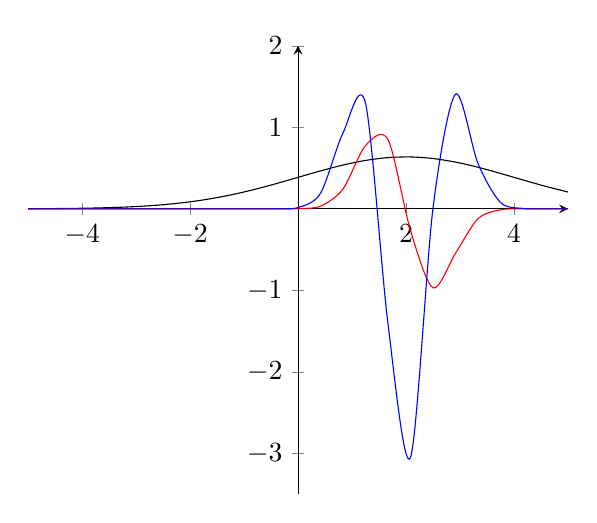
\begin{tikzpicture}
		\begin{axis}[axis lines=left,axis x line=center,axis y line=center,ymax=2,ymin=-3.5]
			\addplot[smooth] {1/(0.5*(0.5*2*3.14))*e^(-(x-2)^2/(2*2^2))};
			\addplot[smooth,red] {(0.002141-0.001071*x)*e^(8*x-2*x^2)};
			\addplot[smooth,blue] {(0.004283*x^2-0.01713*x+0.01606)*e^(8*x-2*x^2)};
		\end{axis}
	\end{tikzpicture} \\\\
	Da $\varphi'(\mu) = 0$ bedeutet das, dass $\varphi(X)$ eine Extremstelle $X=\mu\pm\sigma$ hat.
	Da $\varphi''(\mu) = 0$ bedeutet das, dass $\varphi(X)$ eine Wendestelle $X=\mu\pm\sigma$ hat.
\end{document}